\section{Task Parallel Library}
\subsection{.NET Threads}
\textbf{Keine Vererbung:} Delegate bei Konstruktor.
\textbf{Exception in Thread:} Abbruch des Programs.
\begin{lstlisting}[language=csh]
var myThread = new Thread(() => { /* ... */ });
myThread.start(); /* ... */ myThread.join();
\end{lstlisting}
C\# Lambda kann umgebende Variablen zugreifen (auch scrheibend).

\subsection{Monitor in .NET}
FIFO Warteschlange, Pulse informiert längst Wartenden. \textit{Wait()} in Schlaufe.
\textit{PulseAll()} bi mehreren Bedingungen oder Erfüllungen mehrerer Threads.
Synchronisation mit HilfsObj als Best Practice.
\begin{lstlisting}[language=csh]
private object syncObject = new(); // Monitor auf HilfsObj
public void Widthdraw(decimal amount) {
    lock (syncObject) {
        while(amout > balance) { Monitor.Wait(syncObject); }
        balance -= amount;
    }
}
public void Deposit(decimal amount) {
    lock (syncObject) {
        balance += amount;
        Monitor.PulseAll(syncObject);
    }
}
\end{lstlisting}

\subsection{.NET Synchronisationsprimitiven}
\textbf{Fehlen:} kein Fairnessflag, kein Lock \& Condition.
\textbf{Zusätzlich:} ReadwriteLockSlim für Upgradeable Read/Write. Semaphoren auch auf OS-Stufe nutzbar.
Mutex (binärer Semaphor).
\textbf{Collections nicht Thread-safe:} Ausser \textit{System.Collections.Concurrent}

\subsection{.NET Task Parallel Library (TPL)}
Work Stealing Thread Pool. 
\textbf{Verschiedene Abstraktionsstufen:} Task Parallelization: Explizite Tasks starten und warten.
Data Parallelization: Parallele Statements und Queries.
Asynchrone Programmierung: mit Continuation Style.
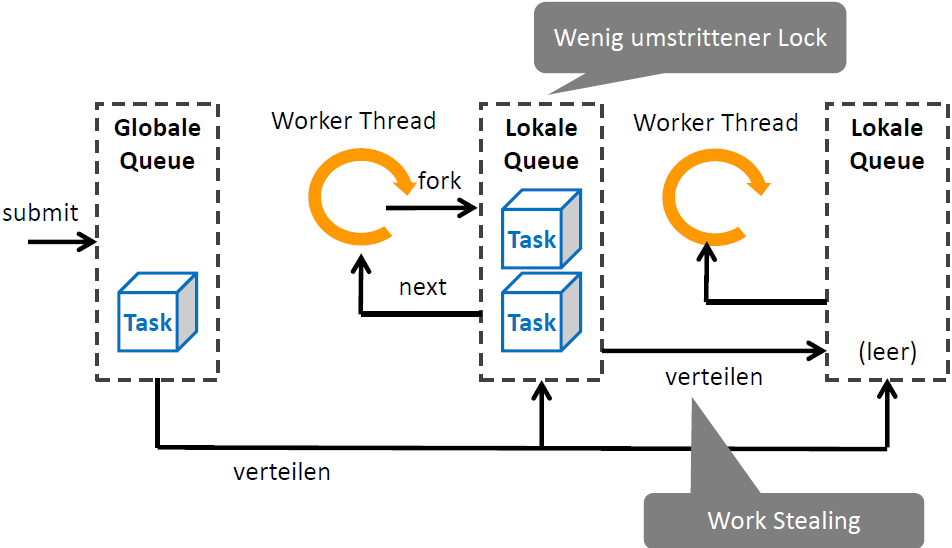
\includegraphics[width=0.7\linewidth]{img/work_stealing_thread_pool.png}

\subsubsection{Thread Injection}
TPL fügt zur Laufzeit neue Worker Threads hinzu.
\textbf{Hill Climbing Algorithmus:} Misst Durchsatz \& variiert Anzahl Worker Threads.
\textbf{Kein Deadlock} bei Task Abhängigkeiten, aber ineffizient, nicht dafür gemacht.

\subsection{Task Parallelisierung}
\begin{lstlisting}[language=csh]
Task task = Task.Run(() => { }); /* ... */ task.Wait();
// Task mit Rueckgabe 
Task<int> task = Task.Run(() => { return 0; });
Console.Write(task.Result); // Blockiert 
// Geschachtelte Tasks
Task.Run(() => {
    var left = Task.Run(() => { }); 
    var right = Task.Run(() => { });
    int res = left.Result + right.Result;
});
\end{lstlisting}

\subsubsection{Parallele Statements}
Menge an Statements potentiell parallel ausführen. Als Task starten. Barriere der Tasks am Ende.
\begin{lstlisting}[language=csh]
Parallel.Invoke(
    () => MergeSort(l, m); () => MergeSort(m,l);
);
\end{lstlisting}

\subsubsection{Parallele Loop}
Schlaufen-Bodies potentiell parallel ausführen.
Gruppierung der Bodies in Tasks.
Berriere dieser Tasks am Ende.
\begin{lstlisting}[language=csh]
Parallel.ForEach(list, file => Convert(file));
Parallel.For(0, array.Length, i => Calc(array[i]));
\end{lstlisting}

\subsubsection{Parallele Loop Partitionierung}
Schlaufe mit vielen sehr kurzen Bodies ist ineffizient.
TPL gruppiert automatisch mehrere Bodies zu Task.
Aufteilung gemäss verfügbaren Worker Threads.\\
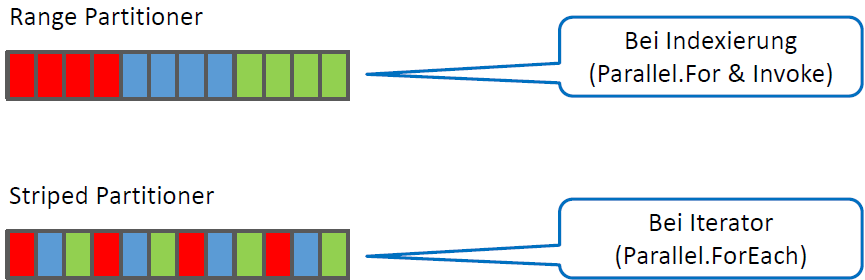
\includegraphics[width=0.7\linewidth]{img/partitionierung.png}\\ 
\textbf{Explizite Partitionierung:} Vorteil: Weniger Body-Delegates, Nachteil: Künstliche Unterschleife.
\begin{lstlisting}[language=csh]
Parallel.ForEach(Partitioner.Create(0, array.Length), 
    (range, _) => {
        for (int i = range.Item1; i < range.Item2; i++) {
            Calc(array[i]);
        }
    })
\end{lstlisting}

\subsection{Parallel LINQ}
Parallelisierung von Langauge-Integrated Query. Pendant zu Java Steam API.
Keyword: \textit{AsParallel()}
\begin{lstlisting}[language=csh]
from book in bookCol.AsParallel()
    where book.Title.Contains("Java") select book.ISBN
\end{lstlisting}

\subsection{Asynchrone Programmierung mit TPL}
\subsubsection{Task Continuation}
\begin{lstlisting}[language=csh]
task1.ContinueWith(task2).ContinueWith(task3);
// Multi-Continuation
Task.WhenAll(task1, task2).ContinueWith(continuation);
Task.WhenAny(task1, task2).ContinueWith(continuation);
\end{lstlisting}